\documentclass[11pt]{article}
\usepackage[utf8]{inputenc}
\usepackage[T5]{fontenc}
\usepackage[margin=1in]{geometry}
\usepackage{float}
\usepackage{xurl}
\usepackage{graphicx}
\usepackage{tikz}
\usepackage{listings}
\usetikzlibrary{arrows.meta, positioning}

\begin{document}

\begin{center}

{\Large \textbf{UNIVERSITY OF SCIENCE AND TECHNOLOGY OF HANOI}}\\
\vspace{0.3cm}
----------------------o0o----------------------\\

\vspace{4cm}

{\large
\centerline{2540027 - Nguyễn Xuân Vinh}
}

\vspace{4cm}

{\Huge \textbf{BC3.04a Advanced Programming for HPC}}\\
\vspace{0.5cm}
Lecturer: Dr. Trần Giang Sơn

\vspace{4cm}

{\Large \textbf{REPORT LABWORK 2}}\\

\vspace{0.5cm}

{\large
Subjects: Get to know your GPU
}

\vspace{4cm}
\today
\end{center}

\newpage
% Cover page here

\newpage

\tableofcontents

\newpage

\section{Objective}

The objective of this labwork is to use \textbf{Numba CUDA} to identify and inspect the GPU available in the computing environment. The information collected includes the GPU device name, device ID, number of multiprocessors, CUDA core information, and GPU memory size.

\section{Environment}

The labwork was performed using \textbf{Google Colab with a cloud GPU runtime}. The Python program uses the numba.cuda module to access and inspect the CUDA device.

\section{GPU Detection}

CUDA availability was first checked using:

\begin{lstlisting}[language=Python]
from numba import cuda
print(cuda.is_available())
\end{lstlisting}

The result was:
\begin{lstlisting}[backgroundcolor=\color{gray!10}]
CUDA available: True
\end{lstlisting}

The available GPU was then detected using:
\begin{lstlisting}[language=Python]
cuda.detect()
\end{lstlisting}

The GPU was selected using:
\begin{lstlisting}[language=Python]
cuda.select_device(0)
\end{lstlisting}

\newpage
\section{GPU Information}

The following information was obtained from the selected GPU:

\begin{figure}[H]
    \centering
    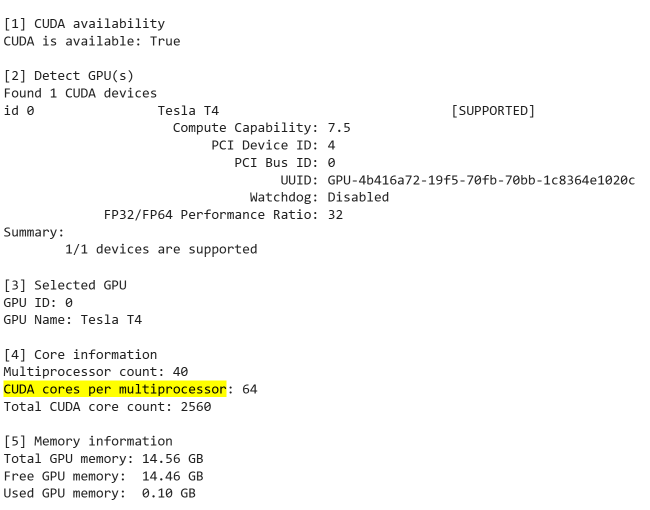
\includegraphics[width=1\textwidth]{img.png}
    \caption{GPU information}
    \label{fig:gpu-infor}
\end{figure}

\section{Conclusion}

This labwork demonstrated how \textbf{Numba CUDA} can be used to access information about an NVIDIA GPU. The program successfully detected the CUDA device, selected the GPU, and retrieved its device name, ID, multiprocessor information, and memory information. The experiment was performed on a \textbf{cloud GPU provided by Google Colab}.

\end{document}